\chapter{Visual Similarity Experiments}
\label{chp:b5}

Image similarity is inherently a subjective phenomenon and like other subjective phenomena user experiments play an important role for a better understanding and improved models. Thus, within the scope of this thesis, a user experiment is conducted to investigate HDR image similarity. This chapter presents the image dataset used for the experiment, the experimental setup that allows the users to assess similarity between HDR image triplets, the data gathering through crowd sourcing and then experiment analysis that displays how the image features introduced in Chapter~\ref{chp:b3} correlates with human responses. Lastly, two models for a combined feature are proposed which is a combination of individual features and the weights of these models are estimated using experiment responses.

\section{Dataset}

The set of images used in visual similarity experiments should be sufficiently diverse. Although such datasets exists for LDR images, there is no specific similarity dataset for HDR images. However, there exists HDR image datasets that were created for various purposes and by different authors. We therefore decided to select 100 HDR images from various such sources to present observers with a diverse set of images2. The used datasets were: Fairchild’s HDR Photographic Survey~\cite{fairchild2007hdr}, HDR-Eye~\cite{nemoto2015visual}, DEIMOS~\cite{klima2011deimos}, Empa HDR Image Database~\cite{EmpaHDR}, and pfstools HDR Image Gallery ~\cite{mantiuk2007high}. Thumbnails for the used images are shown in Figure \ref{fig:dataset}.

\begin{figure}
\begin{center}
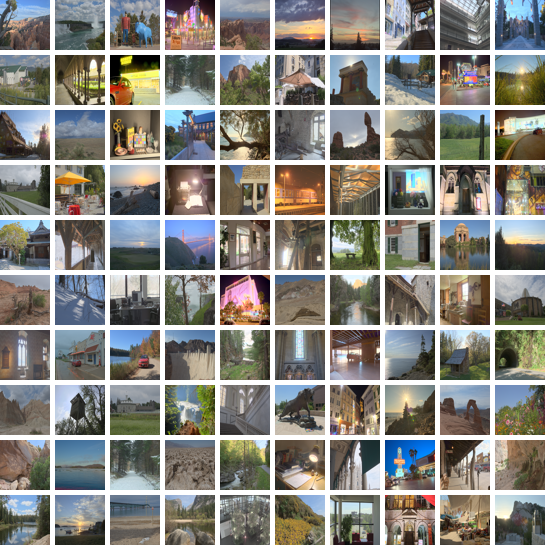
\includegraphics[width=\textwidth]{figures/chapter3/dataset.png}
\caption{HDR images used in the visual similarity experiments.}
\label{fig:dataset}
\end{center}
\end{figure}


\section{Experiment Setting}
%paper
To measure perceptual similarity between HDR images, we conducted a 2AFC experiment. The experiment is publicly available\footnote{http://user.ceng.metu.edu.tr/~merve/userstudy/}. As we needed a large number of responses, we designed a web-based interface to collect crowdsourcing data. We used the HDRHTML technique~\cite{mantiuk2009visualizing} for visualizing HDR images on web browsers.

This technique uses a windowing approach to select a desired exposure range from the HDR image. Multiple exposures are encoded by combining a small set of basis images with opacity coefficients. The tone-curves of these basis images are approximated as a piece-wise linear function. Instead of finding optimal tone-curves and opacity coefficients, HDRHTML uses a precomputed optimal solution and use these tone-curve points and opacity coefficients for all images for fast processing. After basis images are created using the tone-curves, these basis images are used to reconstruct multiple exposures and gives user the control over exposure settings with a slider. By dynamically adjusting the position of the slider, the user can efficiently view the entire exposure range contained within the HDR image. These sliders are normally overlayed with the image histogram. We removed this overlay to prevent the image histogram from affecting the observers’ decisions. Figure \ref{fig:experiment} shows a sample trial from the experiment. An HDR reference image was shown at the top and two HDR test images were shown at the bottom. The sliders, which were mandatory to be adjusted, allowed all images to be inspected at different exposure levels.

\begin{figure}
\begin{center}
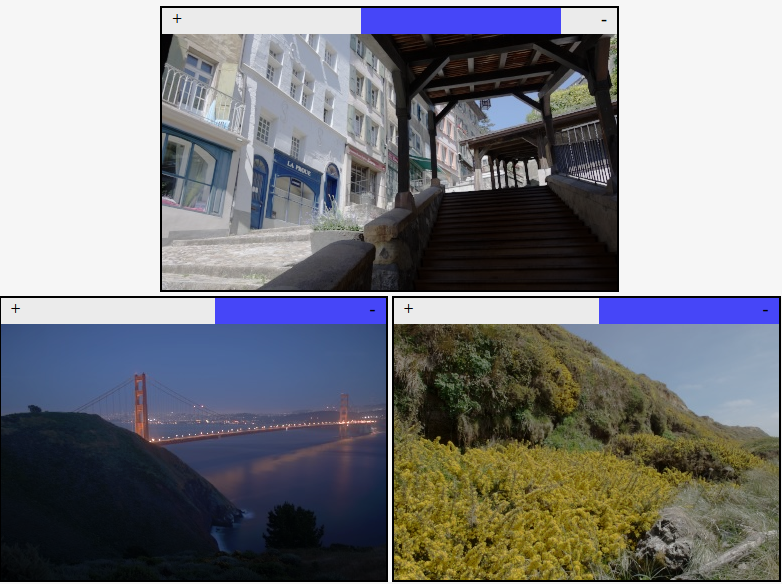
\includegraphics[width=\textwidth]{figures/chapter3/experiment.png}
\caption{A sample trial from the experiment. The observers were asked to choose the most similar image to the reference image (top) from the test images (bottom). All images could be examined at different exposure levels by adjusting their sliders.
%paper
}
\label{fig:experiment}
\end{center}
\end{figure}

In each experimental session, 33 such image triplets were displayed to the observers. Thus, an experimental session consisted of 33 trials. In each trial, the observers were asked to choose which of the two test images was visually more similar to the reference image. All trials, except for the verification ones, were generated randomly from the dataset during the runtime of the experiment. 

Three of the experiment triplets were used for verification. They contained an obviously similar reference and test image pair to evaluate the reliability of an observer as shown in Figure \ref{fig:verficiation}. As seen from the figure, the test image that is similar to the reference image is another image from the same scene. These images are not used in the actual part of the experiment, and do not belong to the dataset of 100 images shown in Figure \ref{fig:dataset}.

\begin{figure}
\begin{center}
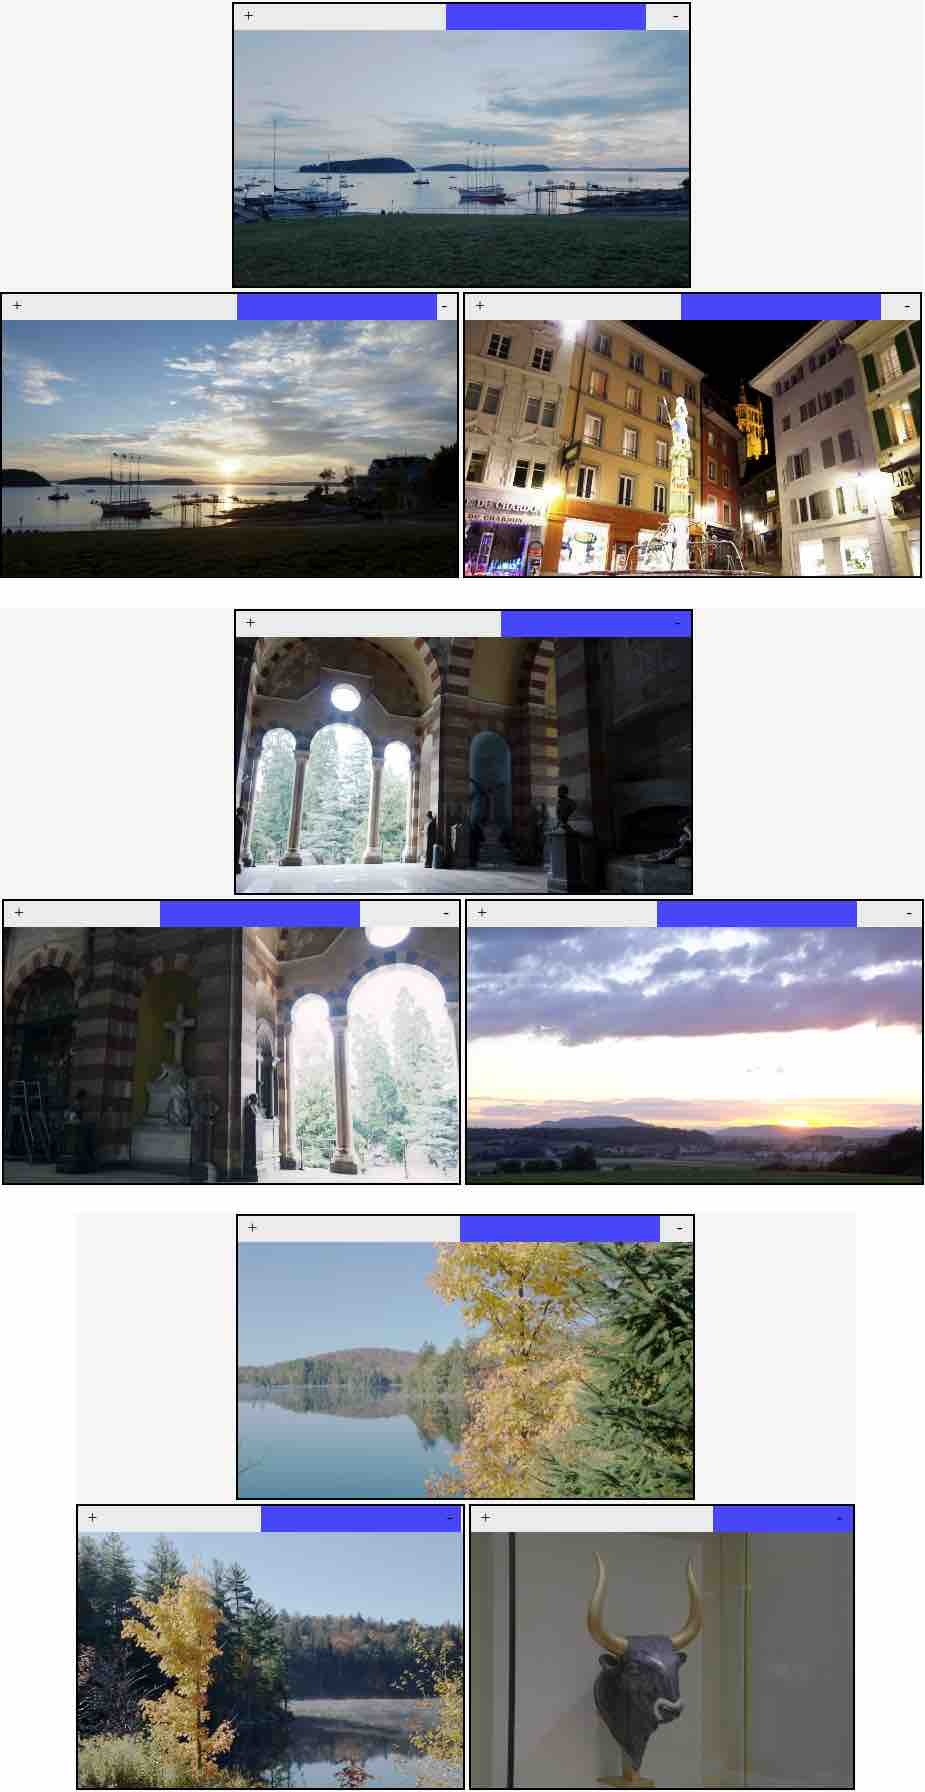
\includegraphics[height=0.85\textheight]{figures/chapter3/verification_small.jpg}
\caption{Verification triplets, shown as 3rd, 10th and 16th trials in the experiment sessions. }
\label{fig:verficiation}
\end{center}
\end{figure}

If an observer failed to provide the correct answer even for one of these trials, his or her data was discarded as being unreliable. These trials were distributed across the experiment to ensure that observers were attentive throughout. Before the experiment began, observers were informed about their task and the expected duration of the experiment, which was at most 20 minutes at a normal pace. During the experiment, observers were required to use the exposure sliders for each image before they made selection. Image selection was done by clicking on one of the test images. The selection was indicated using a green border around the selected image. Observers could change their selection until they pressed the “Next” button. The progress of an observer was indicated using a small progress bar at the bottom center of the screen. At the end of the experiment, observers were informed with a final page confirming the conclusion of the experiment and were presented with unique session ids. They were required to enter this id to the crowdsourcing platform to verify that they have finished the experiment.

\section{Data Collection}
\label{sec:crowd_sourcing}
Crowdsourcing has been used in many computer vision problems to collect non-expert data~\cite{kovashka2016crowdsourcing}. In this thesis, in order to reach as many people as possible, the experiment was published at Microworkers crowdsourcing platform\footnote{www.microworkers.com}. For each completed experiment 0.3\$ were paid to the participants.

At the beginning of the experiment, an introductory page, given in Figure~\ref{fig:experiment_start}, is displayed to the user. This page first describes the task to be fulfilled: complete a set of trials by picking the comparison image that is more similar to the reference image. Here it is important to note that the users are not asked to decide for a specific type of similarity such as object, color, etc. By intentionally leaving the definition of visual similarity vague, it is hoped to achieve a range of responses, which in overall, would converge to a common sense understanding for similarity.
\begin{figure}
\begin{center}
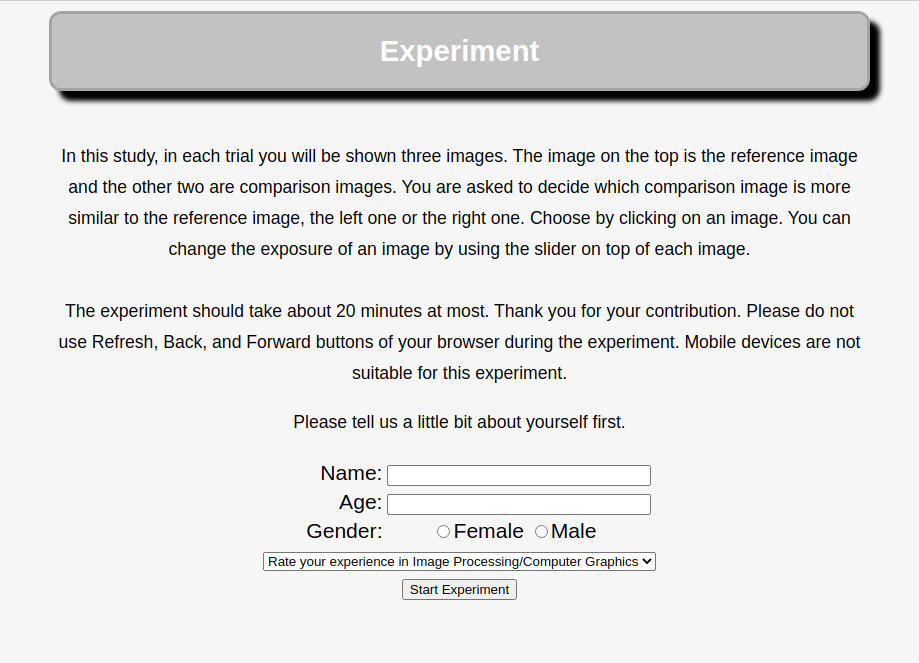
\includegraphics[width=0.85\textwidth]{figures/chapter3/experiment_start.png}
\caption{Start page of the experiment, that describes the task and collects some information about the user.}
\label{fig:experiment_start}
\end{center}
\end{figure}

After giving the instructions about the experiment, the user is informed about the expected time to finish the experiment when done in a normal pace. This is followed by some warnings about browser usage during the experiment and unsuitable devices. Then, a form is presented to collect some information about the participants. In Figure~\ref{fig:age_gender_cgi}, the distribution of age, gender, and familiarity with computer graphics/image processing of the participants according to the data entered to this form is shown. Finally, the user can start the experiment on demand by pressing the provided button labeled as "Start Experiment".

\begin{figure}
\begin{center}
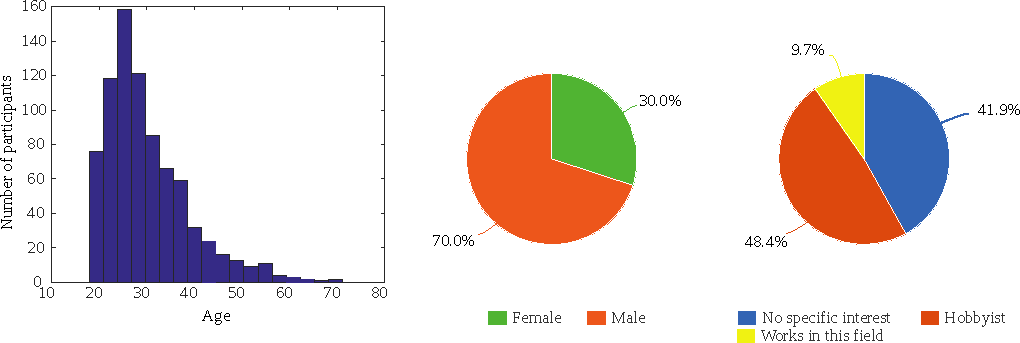
\includegraphics[width=\textwidth]{figures/chapter3/age_gender_cgi.pdf}
\caption{Age, gender, and computer graphics/image processing familiarity distribution of the participants.}
\label{fig:age_gender_cgi}
\end{center}
\end{figure}

One of the challenges of data crowdsourcing is eliminating users that give unreliable responses, this may due to not being qualified for the task or just being a spammer~\cite{garcia2016challenges}. To minimize the problem of users being not qualified, the crowd group of English speaking, highly qualified users are selected from the crowdsourcing platform. Even though the experiment itself does not require language proficiency, the instructions at the beginning of the experiment is important for users to successfully complete the experiment. The users are in the \emph{highly qualified} crowd, if they have been done other crowdsourcing tasks before and received some positive feedback. Another measure taken to achieve reliable responses is using verification triplets. In total, 165 sessions were discarded due to incorrect responses given to the verification trials. 

\subsection{Phase I}
\label{sec:exp_phase_I}
In the first phase of the experiment, randomly selected triplets are shown to the users without any restrictions on the image selection. After collecting the experimental results, and eliminating the triplets from invalid sessions, it was found that 18747 unique image triplets were judged by the observers. This amounts to approximately 11.6\% of the total possible triplets that can be obtained from 100 images, $C(100, 3)$. Experiment sessions were independent and random for each participant, but it was guaranteed that a single session consisted of only unique triplets. 

This design resulted in a single response for the majority of the triplets. Some triplets received two responses and only a few received three or more. As such this first phase of the experiment is considered as a random exploration of all possible comparisons. However, as judging similarity based on a single response could be too subjective, the experiment is extended as discussed below to collect multiple responses for each triplet.

\subsection{Phase II}
\label{sec:exp_phase_II}
The first phase of the experiment was extended to obtain three evaluations per triplet. Unlike the first phase where triplets were generated randomly, the second phase solely used the triplets that had been evaluated in the first phase of the experiment. To achieve this, the triplets sorted from the first phase in descending order by the number of responses collected. If a triplet had more than three responses, three of the responses are randomly selected. The triplets with exactly three responses were used as is. These two cases occurred very rarely. Next, triplets with two responses, and then a single response were presented randomly to obtain a total of 4990 triplets that had been evaluated three times. Among these thrice evaluated triplets, 2170 triplet were judged consistently by all three observers. The remaining 2820 triplets generated two-to-one responses. Similar to the first part of the experiment, the second part also contained the same validity checks to eliminate the responses of inattentive observers.

\section{Experiment Analysis}

Having discussed the details of crowdsourcing study in Section \ref{sec:crowd_sourcing} and experimented features in Section \ref{sec:features}, this section investigates how the human judgments and the image features are related. First analysis method for assessing the correlation between individual feature type and the experiment results is given. Then, two possible methods to combine the features for developing a more effective similarity model is discussed. In the evaluations, different formats for HDR images are employed in order to measure the effect of the image format to the proposed methods. 

\subsection{Preprocessing}
In evaluations, HDR images used directly, as well as by linear scaling and applying several tone mapping operators. For linear scaling, 5\% of the brightest pixels and 5\% of the darkest pixels are discarded by setting them to 95th and 5th percentile of the pixels values respectively. The reason behind this step is to eliminate extreme values from the HDR images that may also introduced by hardware. 

\begin{equation}
    I' = \begin{cases}
    P_5 (I), &\text{ if $I < P_5(I)$} \\
    I, &\text{ if $P_5(I) \leq I \leq P_{95}(I) $} \\
    P_{95}(I), &\text{if $I > P_{95}(I)$}, \\
    \end{cases}
\end{equation}

where $I$ denotes the original image values and $I'$ is after the pixel values outside of the range are removed. Then HDR image is linearly scaled with

\begin{equation}
    lin(I)  = {{I' - I'_{min}} \over {I'_{max} - I'_{min}}}, 
\end{equation}

for each color channel separately.

Besides of using original and linearly scaled HDR images, tone mapped version of the images are also evaluated. For this purpose commonly used tone mapping operators Mai et al. ~\cite{mai2010optimizing}, Reinhard et al. (local) ~\cite{reinhard2002photographic}, Reinhard et al. (global) ~\cite{reinhard2002photographic}, Durand \& Dorsey~\cite{durand2002fast}, Mantiuk et al.~\cite{mantiuk2006perceptual}, Reinhard \& Devlin~\cite{reinhard2005dynamic}, Fattal et al.~\cite{durand2002fast}, Mantiuk et al.~\cite{mantiuk2008display}, Ferradans et al.~\cite{ferradans2011analysis} and Pattanaik et al.~\cite{pattanaik2000time} are used. The implementations of these TMOs are available in opensource PFStmo software library ~\cite{mantiuk2007high}, which provides a reliable implementation of several commonly used TMOs. The images in the experiment dataset are tone mapped using the PFStmo software with the given TMOs using the default parameters.


\subsection{Individual Feature Correlations}
To investigate how individual image features correlate with the human responses collected through the experiment, the feature responses are treated as an observer that are given the same set image triplets used in the experiment. Assume that $t_i = R_i-A_i-B_i$ represents the $i^{th}$ triplet (i.e. trial) with $R_i$ being the reference image, $A_i$ the left test image, and $B_i$ the right test image. This triplet could have been evaluated one or more times by different human observers. Let $n(A_i)$ and $n(B_i)$ represent the number of times that each image was found more similar to $R_i$ than the other. From this information, a binary vector is created to encode the participants’ responses:
\begin{equation}
\label{eq:p_vector}
P = (x_1, \ldots, x_N),
\end{equation}

where each element is defined as:
\begin{equation}
x_i = \begin{cases}
1, &\text{if $n(A_i) > n(B_i)$}, \\
0, &\text{otherwise}.
\end{cases}
\end{equation}

For each feature type $f$, the feature representations of each image is computed as $f(R_i)$, $f(A_i)$, $f(B_i)$. Then their similarity to each other is calculated to obtain the following binary vector:
\begin{equation}
    F = (y_1,\cdots, y_N ),
\end{equation}
where
\begin{equation}
y_i = \begin{cases}
1, &\text{ if $ d(f(R_i), f(A_i)) < d(f(R_i), f(B_i))$ } \\
0, &\text{otherwise}.
\end{cases}
\end{equation}

In this equation $d$ represents the distance metric that was chosen to be used for feature $f$. This encoding gave rise to two binary vectors, $P$ and $F$, with the former computed from user responses and the latter from feature similarities. There are many approaches to compute the correlation between two such vectors. In this thesis, the Sokal-Michener correlation is used, which is a simple, intuitive, and effective way to correlate two binary vectors~\cite{zhang2003properties}. This correlation is defined as

\begin{equation}
s = {{S_{11}(P, F) + S_{00}(P, F)} \over {N}},
\end{equation}

with $S_{11}$ and $S_{00}$ representing the total count of matching ones and zeros respectively:

\begin{align}
    S_{11}(P, F) &= P \cdot F,\\
    S_{00}(P, F) &= \neg P \cdot \neg F, 
\end{align}


Note that the correlation coefficient s can take a value in range [0, 1]. In the following, this coefficient is multiplied by 100 to represent the correlations as percentages.

The raw feature correlations with the first (Section \ref{sec:exp_phase_I}) and the second phase of the experiment (Section \ref{sec:exp_phase_II}) are reported in Tables \ref{tab:ind_correlation_p1} and \ref{tab:ind_correlation_p2}, respectively. In these tables, the leftmost column indicates the processing type applied to the images before the computation of features.

\afterpage{
\begin{landscape}
\begin{table}
\caption{Individual feature correlations with the first phase of the experiment. The numbers indicate the Sokal-Michener correlation scaled by 100 to represent percentages.}
\centering
\begin{tabular}{r | c c c c c c c}
\label{tab:ind_correlation_p1}
\textbf{Processing Type} & \textbf{VGG16} & \textbf{VGG19} & \textbf{Color} & \textbf{Luminance} & \textbf{Texture} & \textbf{GIST}\\
\hline
HDR-original & 56.79 & 58.09 & 55.10 & 53.14 & 52.39 & 56.82 \\
HDR-linear & 63.54 & 63.31 & 55.69 & 54.07 & 54.36 & 58.18 \\
Drago et al.~\cite{drago2003adaptive} & 65.88 & 65.74 & 56.73 & 57.45 & 51.17 & 58.23 \\
Mai et al.~\cite{mai2010optimizing} & 65.28 & 65.13 & 56.01 & 56.77 & 51.90 & 57.57 \\ 
Reinhard et al. (local)~\cite{reinhard2002photographic} & 65.82 & 65.63 & 56.58 & 54.77 & 51.43 & 57.89 \\
Reinhard et al. (global)~\cite{reinhard2002photographic} & 65.75 & 65.52 & 56.59 & 54.68 & 51.39 & 57.92 \\
Durand \& Dorsey~\cite{durand2002fast} & 66.17 & 65.43 & 55.77 & 55.12 & 51.79 & 57.85 \\
Mantiuk et al.~\cite{mantiuk2006perceptual} & 65.42 & 65.33 & 56.29 & 55.38 & 52.08 & 58.03 \\
Reinhard \& Devlin~\cite{reinhard2005dynamic} & 65.28 & 65.20 & 57.15 & 55.89 & 54.85 & 58.33 \\
Fattal et al.~\cite{durand2002fast} & 65.90 & 65.72 & 56.39 & 57.46 & 51.92 & 58.19 \\
Mantiuk et al.~\cite{mantiuk2008display} & 65.71 & 65.74 & 55.98 & 56.99 & 51.84 & 57.86 \\
Ferradans et al.~\cite{ferradans2011analysis} & 66.02 & 65.90 & 55.18 & 56.51 & 51.99 & 58.33 \\
Pattanaik et al.~\cite{pattanaik2000time} & 64.46 & 64.38 & 53.04 & 54.61 & 53.06 & 57.84 
\end{tabular}
\end{table}
\end{landscape}
}

\afterpage{
\begin{landscape}
\begin{table}
\caption{Individual feature correlations with the second phase of the experiment. The numbers indicate the Sokal-Michener correlation scaled by 100 to represent percentages.}
\centering
\begin{tabular}{r|c c c c c c c}
\label{tab:ind_correlation_p2}
\textbf{Processing Type} & \textbf{VGG16} & \textbf{VGG19} & \textbf{Color} & \textbf{Luminance} & \textbf{Texture} & \textbf{GIST}\\
\hline
HDR-original & 64.88 & 67.14 & 60.23 & 58.39 & 54.42 & 63.50 \\
HDR-linear & 75.58 & 76.13 & 60.78 & 57.79 & 57.97 & 65.71 \\
Drago et al.~\cite{drago2003adaptive} & 80.88 & 81.80 & 62.58 & 62.72 & 53.87 & 65.39 \\
Mai et al.~\cite{mai2010optimizing} & 80.00 & 79.95 & 61.11 & 61.66 & 53.46 & 64.06 \\
Reinhard et al. (local)~\cite{reinhard2002photographic} & 80.92 & 81.61 & 62.21 & 58.16 & 53.87 & 64.88 \\
Reinhard et al. (global)~\cite{reinhard2002photographic} & 80.92 & 81.57 & 62.21 & 57.97 & 54.75 & 64.75 \\
Durand \& Dorsey~\cite{durand2002fast} & 81.75 & 81.34 & 62.07 & 59.22 & 53.00 & 64.19 \\
Mantiuk et al.~\cite{mantiuk2006perceptual} & 80.41 & 80.65 & 61.15 & 59.59 & 52.49 & 64.47 \\ 
Reinhard \& Devlin~\cite{reinhard2005dynamic} & 80.37 & 80.41 & 64.15 & 61.43 & 60.55 & 65.44 \\
Fattal et al.~\cite{durand2002fast} & 80.51 & 80.92 & 62.30 & 64.24 & 52.90 & 65.02 \\
Mantiuk et al.~\cite{mantiuk2008display} & 80.00 & 80.78 & 62.12 & 61.71 & 54.56 & 64.19 \\
Ferradans et al.~\cite{ferradans2011analysis} & 81.38 & 82.21 & 58.39 & 61.61 & 55.02 & 65.25 \\
Pattanaik et al.~\cite{pattanaik2000time} & 78.66 & 78.11 & 57.33 & 58.66 & 55.71 & 64.52
\end{tabular}
\end{table}
\end{landscape}
}

“HDR-original” represents the unaltered HDR image whereas “HDR-linear” represents its linearly scaled version. The other processing types all include the application of a certain tone mapping operator. For all processing types, except the original, the images were gamma-corrected and scaled to [0, 255] range.

%In both models, closely related deeply learned features VGG16 and VGG19 used as separate features instead of selecting the better performing one. The reason behind this, as the study~\cite{simonyan2014very} suggests, the results obtained from combination of VGG16 and VGG19 (by taking an average) performs better than both VGG16 and VGG19, indicates that VGG16 and VGG19 are complementary features. This claim is consistent with the results given Table \ref{tab:fuse_vgg_phaseI_II}, although the improvement is not high.

%\afterpage{
%\begin{landscape}
%\begin{table}
%\caption{Comparison of correlation results for the features VGG16, VGG19 and combination VGG16-19 for the Phase I (left half) and Phase II (right half) of the experiment.}
%\label{tab:fuse_vgg_phaseI_II}
%\begin{tabular}{r|c|c|c||c|c|c}
%\textbf{Processing Type} & \textbf{VGG16} & \textbf{VGG19} & \textbf{VGG16-19} & \textbf{VGG16} & \textbf{VGG19} & \textbf{VGG16-19} \\
%\hline
%HDR-original &  56.79 & 58.09 & 57.91 &  64.88  &  67.14  &  66.59\\
%HDR-linear &  63.54 & 63.31 & 63.85 &  75.58   & 76.13 & 76.96 \\
%Drago et al.~\cite{drago2003adaptive} &  65.88 & 65.74 & 66.31 &  80.88 &    81.8 &    82.35\\
%Mai et al.~\cite{mai2010optimizing} &  65.28 & 65.13 & 66.06 &  80.00 &   79.95    & 81.20 \\
%Reinhard et al. (local)~\cite{reinhard2002photographic} & 65.82 & 65.63 & 66.21 & 80.92 &    81.61 &    82.21 \\
%Reinhard et al. (global)~\cite{reinhard2002photographic} & 65.75 & 65.52 & 66.29 & 80.92   & 81.57   &  82.30 \\
%Durand \& Dorsey~\cite{durand2002fast} & 66.17 & 65.43 & 66.44 & 81.75   & 81.34  &  82.76 \\
%Mantiuk et al.~\cite{mantiuk2006perceptual} & 65.42 & 65.33 & 65.97 & 80.41   & 80.65 &   81.24 \\
%Reinhard \& Devlin~\cite{reinhard2005dynamic} & 65.28 & 65.20 & 65.81 & 80.37  &  80.41 & 81.24\\
%Fattal et al.~\cite{durand2002fast} & 65.90 & 65.72 & 66.25 & 80.51 & 80.92 & 81.98\\
%Mantiuk et al.~\cite{mantiuk2008display} & 65.71 & 65.74 & 66.01 &  80.00   & 80.78 & 80.51\\
%Ferradans et al.~\cite{ferradans2011analysis} & 66.02 & 65.90 & 66.77 & 81.38 & 82.21 &  83.27\\
%Pattanaik et al.~\cite{pattanaik2000time} & 64.46 & 64.38 & 64.76 & 78.66   & 78.11   & 79.77
%\end{tabular}
%\end{table}
%\end{landscape}
%}


\subsection{Statistical Analysis}
In Table~\ref{tab:p_individual}, the statistical significance of the difference between each individual feature correlations are given. Fisher's exact test~\cite{fisher1922interpretation} is used for the calculations, image features are calculated on images tone mapped with Ferradans et al.~\cite{ferradans2011analysis} TMO, and correlation is calculated against Phase II of the experiment. This analysis shows that, the difference for the correlations of VGG16 and VGG19 features are not that significant and also Color - Luminance - Texture performances are rather close. On the other hand, deep learning features are significantly better than the other features and similarly, GIST feature is significantly better than Color and Texture features.


\begin{table}
\caption{$p$ values for statistical significance between individual image features, calculated with Fisher's exact test.}
\label{tab:p_individual}
\centering
\resizebox{\textwidth}{!}{\begin{tabular}{c | c c c c c c}
 &VGG16& VGG19& Color& Luminance& Texture & GIST \\
\hline
VGG16 & $1.0$ & $0.504$ & $3.832x10^{-62}$ &$1.123x10^{-47}$ &$4.828x10^{-79}$ &$1.963x10^{-33}$ \\
VGG19 & $0.504$ & $1.0$ & $3.083x10^{-67}$ & $3.670x10^{-52}$ & $9.416x10^{-85}$ &$3.302x10^{-37}$ \\
Color & $3.832x10^{-62}$ &$3.083x10^{-67}$ &$1.0$ &$0.033$ &$0.027$ &$3.720x10^{-06}$ \\
Luminance & $1.123x10^{-47}$ &$3.670x10^{-52}$ &$0.033$ &$1.0$ &$1.222x10^{-05}$ &$0.014$ \\
Texture & $4.828x10^{-79}$ &$9.416x10^{-85}$ &$0.027$ &$1.222x10^{-05}$ &$1.0$ &$6.947x10^{-12}$ \\
GIST &$1.963x10^{-33}$ &$3.302x10^{-37}$ &$3.720x10^{-06}$ &$0.014$ &$6.947x10^{-12}$ &$1.0$  
\end{tabular}}
\end{table}

Another variable in the experiment analysis is the selection of tone mapping operators. Results given in Table~\ref{tab:ind_correlation_p1} and Table~\ref{tab:ind_correlation_p2} shows that for a given image feature tone mapping operators are performing comparably. Table~\ref{tab:p_tmos} shows the $p$ values calculated with Fisher's exact test~\cite{fisher1922interpretation} between the VGG19 feature's correlation with the Phase II of the user study on images tone mapped with different tone mapping operators. While for most of the tone mapping operators the performance difference is not significant. For this feature, the differences between the best performing Ferradans et. al.'s TMO~\cite{ferradans2011analysis} and the successors Drago et al.'s~\cite{drago2003adaptive} and Reinhard et al.~\cite{reinhard2002photographic} TMOs are not significant ($p > 0.6$). However, the difference to the worst performing TMO, Pattanaik et al.'s TMO is significant with $p=0.001$.

\begin{table}[ht]
\caption{$p$ values for statistical significance between correlations of VGG19 features extracted on images tone mapped with different tone mapping operators, calculated with Fisher's exact test. User responses are used from Phase II of the experiment.}
\label{tab:p_tmos}
\resizebox{\textwidth}{!}{\begin{tabular}{c|c c c c c }
\centering
 & Dra.~\cite{drago2003adaptive} & Mai.~\cite{mai2010optimizing} & Rein.(local)~\cite{reinhard2002photographic} & Rein. (global)~\cite{reinhard2002photographic} & Dur.~\cite{durand2002fast} \\
\hline
Dra.~\cite{drago2003adaptive} & 1.0 &0.132 &0.906 &0.875 &0.725  \\ 
Mai.~\cite{mai2010optimizing} & 0.132 &1.0 &0.178 &0.19 &0.265  \\ 
Rein.(local)~\cite{reinhard2002photographic} & 0.906 &0.178 &1.0 &1.0 &0.845 \\ 
Rein.(global)~\cite{reinhard2002photographic} & 0.875 &0.19 &1.0 &1.0 &0.876  \\ 
Dur.~\cite{durand2002fast} & 0.725 &0.265 &0.845 &0.876 &1.0  \\ 
Man.~\cite{mantiuk2006perceptual} & 0.351 &0.593 &0.438 &0.461 &0.588  \\ 
Rein.~\cite{reinhard2005dynamic} & 0.261 &0.732 &0.333 &0.353 &0.463  \\ 
Dur.~\cite{durand2002fast} & 0.483 &0.444 &0.586 &0.613 &0.756  \\ 
Man.~\cite{mantiuk2008display} & 0.414 &0.516 &0.509 &0.534 &0.67  \\ 
Fer.~\cite{ferradans2011analysis} & 0.752 &0.063 &0.636 &0.608 &0.479  \\ 
Pat.~\cite{pattanaik2000time} & 0.003 &0.146 &0.005 &0.005 &0.009\\ 
\end{tabular}}
\\
\\
\\
\resizebox{\textwidth}{!}{\begin{tabular}{c|c c c c c c}
\centering
  & Man.~\cite{mantiuk2006perceptual} & Rein.~\cite{reinhard2005dynamic} & Dur.~\cite{durand2002fast} & Man.~\cite{mantiuk2008display} & Fer.~\cite{ferradans2011analysis} & Pat.~\cite{pattanaik2000time}\\
\hline
Dra.~\cite{drago2003adaptive} &0.351 &0.261 &0.483 &0.414 &0.752 &0.003 \\ 
Mai.~\cite{mai2010optimizing} &0.593 &0.732 &0.444 &0.516 &0.063 &0.146 \\ 
Rein.(local)~\cite{reinhard2002photographic} &0.438 &0.333 &0.586 &0.509 &0.636 &0.005 \\ 
Rein.(global)~\cite{reinhard2002photographic}  &0.461 &0.353 &0.613 &0.534 &0.608 &0.005 \\ 
Dur.~\cite{durand2002fast}  &0.588 &0.463 &0.756 &0.67 &0.479 &0.009 \\ 
Man.~\cite{mantiuk2006perceptual} &1.0 &0.878 &0.847 &0.939 &0.198 &0.043 \\ 
Rein.~\cite{reinhard2005dynamic}  &0.878 &1.0 &0.701 &0.788 &0.139 &0.067 \\ 
Dur.~\cite{durand2002fast}  &0.847 &0.701 &1.0 &0.939 &0.291 &0.024 \\ 
Man.~\cite{mantiuk2008display} &0.939 &0.788 &0.939 &1.0 &0.241 &0.032 \\ 
Fer.~\cite{ferradans2011analysis}  &0.198 &0.139 &0.291 &0.241 &1.0 &0.001 \\ 
Pat.~\cite{pattanaik2000time}  &0.043 &0.067 &0.024 &0.032 &0.001 &1.0 \\ 
\end{tabular}}
\end{table}


%\begin{landscape}
%\begin{table}[ht]
%\resizebox{\textheight}{!}{\begin{tabular}{c|c c c c c c c c c c c}
%\centering
% & Drago et al.~\cite{drago2003adaptive} & Mai et al.~\cite{mai2010optimizing} & Reinhard et al. (local)~\cite{reinhard2002photographic} & Reinhard et al. (global)~\cite{reinhard2002photographic} & Durand \& Dorsey~\cite{durand2002fast} & Mantiuk et al.~\cite{mantiuk2006perceptual} & Reinhard \& Devlin~\cite{reinhard2005dynamic} & Fattal et al.~\cite{durand2002fast} & Mantiuk et al.~\cite{mantiuk2008display} & Ferradans et al.~\cite{ferradans2011analysis} & Pattanaik et al.~\cite{pattanaik2000time}\\
%\hline
%Drago et al.~\cite{drago2003adaptive} & 1.0 &0.132 &0.906 &0.875 &0.725 &0.351 &0.261 &0.483 &0.414 &0.752 &0.003 \\ 
%Mai et al.~\cite{mai2010optimizing} & 0.132 &1.0 &0.178 &0.19 &0.265 &0.593 &0.732 &0.444 &0.516 &0.063 &0.146 \\ 
%Reinhard et al. (local)~\cite{reinhard2002photographic} & 0.906 &0.178 &1.0 &1.0 &0.845 &0.438 &0.333 &0.586 &0.509 &0.636 &0.005 \\ 
%Reinhard et al. (global)~\cite{reinhard2002photographic} & 0.875 &0.19 &1.0 &1.0 &0.876 &0.461 &0.353 &0.613 &0.534 &0.608 &0.005 \\ 
%Durand \& Dorsey~\cite{durand2002fast} & 0.725 &0.265 &0.845 &0.876 &1.0 &0.588 &0.463 &0.756 &0.67 &0.479 &0.009 \\ 
%Mantiuk et al.~\cite{mantiuk2006perceptual} & 0.351 &0.593 &0.438 &0.461 &0.588 &1.0 &0.878 &0.847 &0.939 &0.198 &0.043 \\ 
%Devlin~\cite{reinhard2005dynamic} & 0.261 &0.732 &0.333 &0.353 &0.463 &0.878 &1.0 &0.701 &0.788 &0.139 &0.067 \\ 
%Fattal et al.~\cite{durand2002fast} & 0.483 &0.444 &0.586 &0.613 &0.756 &0.847 &0.701 &1.0 &0.939 &0.291 &0.024 \\ 
%Mantiuk et al.~\cite{mantiuk2008display} & 0.414 &0.516 &0.509 &0.534 &0.67 &0.939 &0.788 &0.939 &1.0 &0.241 &0.032 \\ 
%Ferradans et al.~\cite{ferradans2011analysis} & 0.752 &0.063 &0.636 &0.608 &0.479 &0.198 &0.139 &0.291 &0.241 &1.0 &0.001 \\ %Pattanaik et al.~\cite{pattanaik2000time} & 0.003 &0.146 &0.005 &0.005 &0.009 &0.043 &0.067 &0.024 &0.032 &0.001 &1.0 \\ 
%\end{tabular}}
%\caption{caption[!]}
%\end{table}
%\end{landscape}


\subsection{Combined Feature Correlation}

Given the individual correlations reported in the previous tables Table~\ref{tab:ind_correlation_p1} and Table~\ref{tab:ind_correlation_p2}, a natural question that follows is if the features can be combined to develop a single objective metric that better correlates with human’s assessment of similarity for HDR images. To this end, two types of logistic regression analysis are performed yielding two related but different models.

%\begin{table}
%\caption{Comparison of correlation results for the features VGG16, VGG19 and combination VGG16-19 for the Phase II of the experiment}
%\label{tab:fuse_vgg_phaseII}
%\begin{tabular}{c|c|c|c}
%\textbf{Processing Type} & \textbf{VGG16} & \textbf{VGG19} & \textbf{VGG16-19} \\
%\hline
%HDR-original &  64.88  &  67.14  &  66.59 \\
%HDR-linear &  75.58   & 76.13 & 76.96 \\
%Drago et al. ~\cite{drago2003adaptive} &  80.88 &    81.8 &    82.35 \\
%Mai et al. ~\cite{mai2010optimizing} &  80 &   79.95    & 81.2 \\
%Reinhard et al. (local) ~\cite{reinhard2002photographic} & 80.92 &    81.61 &    82.21 \\
%Reinhard et al. (global) ~\cite{reinhard2002photographic} & 80.92   & 81.57   &  82.3 \\
%Durand \& Dorsey~\cite{durand2002fast} & 81.75   & 81.34  &  82.76 \\
%Mantiuk et al.~\cite{mantiuk2006perceptual} & 80.41   & 80.65 &   81.24 \\
%Reinhard \& Devlin~\cite{reinhard2005dynamic} & 80.37  &  80.41 &    81.24 \\
%Fattal et al.~\cite{durand2002fast} & 80.51   & 80.92 &    81.98 \\
%Mantiuk et al.~\cite{mantiuk2008display} &  80   & 80.78   & 80.51 \\
%Ferradans et al.~\cite{ferradans2011analysis} & 81.38 &    82.21 &    83.27 \\
%Pattanaik et al.~\cite{pattanaik2000time} & 78.66   & 78.11   & 79.77
%\end{tabular}
%\end{table}



\subsubsection{Triplet Model}
In the first analysis, the aim is to develop a model that predicts which of the two test images is more similar to the reference image using the pairwise distances between the test and reference images. Assuming that j is a feature index, one can compute these pairwise differences as follows:
\begin{align}
    a_j &= d_j(f_j(R), f_j(A)), \\
   b_j &= d_j(f_j(R), f_j(B)). 
\end{align}

Here $d_j$ represents the distance metric chosen for the $j^{th}$ feature. The model takes as input these differences for all features (i.e. $j \in {1, 2, 3, 4, 5, 6}$) and computes their weighted average as its response:

\begin{equation}
    r = c_0 + c_1(a_1 - b_1) + c_2(a_2 - b_2) + c_3(a_3 - b_3)+ c_4(a_4 - b_4) + c_5(a_5 - b_5) + c_6(a_6 - b_6)
\end{equation}
 

To compute the unknown coefficients logistic regression is used as the dependent data (i.e. user responses)
is binary: given one reference and two test images, the user selects either the left image or the right one,
encoded as 1 and 0.

The regression is performed between the two vectors, namely the $P$ vector from Equation \ref{eq:p_vector}, and the model response $R$ comprised of the following elements:
\begin{equation}
    R = (r_1,\cdots, r_N ),
\end{equation}
where
\begin{equation}
    r_i = [a_{i1} - b_{i1} \cdots a_{i6} - b_{i6}].
\end{equation}

The logistic regression models the logarithm of the odds as the response of the model:
\begin{equation}
   ln \left( {{Pr(x = 1)} \over { 1 - Pr(x = 1)}} \right) = r. 
\end{equation}


From this equation, it can be derived that the probability of a user responding 1 (i.e. selecting the left image) is equal to

\begin{equation}
\label{eq:response_prob}
    Pr(x = 1) = {{1} \over {1 + e^{-r}}}
\end{equation}

If $Pr(x = 1) > 0.5$, it is assumed that the model has selected the left image. Otherwise, the model’s response was taken as the right image.

To measure the effectiveness of this model 10-fold cross validation is used. In each fold, 90\% of the trials were selected for training and the remaining 10\% for testing. This process was repeated 10 times while ensuring that each test fold is mutually exclusive from each other. Similar to the analysis of individual features, the success of this model is assessed against both the Phase I and the Phase II of the experiment. The results are shown in Table \ref{tab:correlation_triplet_model}. It can be seen that the feature combination, on average, improves the success of each presentation type by about 3\% to 4\%. The best three results are obtained by Ferradans et al.’s~\cite{ferradans2011analysis}, Drago et al.’s~\cite{drago2003adaptive}, and Reinhard et al.’s ~\cite{reinhard2002photographic} TMO algorithms. The reported coefficients are computed by using the entire dataset from the Phase II of the experiment due to its higher correlation with the combined features.

\afterpage{
\begin{landscape}
\begin{table}
\caption{The correlations of the first regression model with the user responses. Phase I and Phase II represent the initial and extended experiments respectively. The coefficients are reported for the Phase II of the experiment only due to its higher correlation with the user data.}
\centering
\begin{tabular}{r|c c || r r r r r r r}
\label{tab:correlation_triplet_model}
\textbf{Processing Type} & \textbf{Phase I} & \textbf{Phase II} & \textbf{c0} & \textbf{c1} & \textbf{c2} & \textbf{c3} & 
\textbf{c4} & \textbf{c5} & \textbf{c6}\\
\hline
HDR-original & 60.67 & 70.76 & 0.0573 & 0.0768 & -3.3241 & -0.0028 & -0.0124 & -0.2921 & -10.7505 \\
HDR-linear & 64.81 & 78.83 & 0.0005 & -5.4801 & -5.9902 & -0.0074 & -0.0635 & -0.3289 & -10.1782 \\
Drago et al. ~\cite{drago2003adaptive} & 67.36 & 83.49 & -0.0423 & -7.8751 & -7.6339 & -0.0506 & -0.0958 & 0.0043 & -7.3615 \\
Mai et al. ~\cite{mai2010optimizing} & 66.70 & 81.78 & 0.0085 & -5.2932 & -7.9526 & -0.0601 & -0.1078 & -0.0358 & -4.9275 \\
Reinhard et al. (local) ~\cite{reinhard2002photographic} & 67.19 & 83.21 & -0.0154 & -7.3838 & -8.7207 & -0.0688 & -0.0853 & 0.0145 & -7.8380 \\
Reinhard et al. (global) ~\cite{reinhard2002photographic} & 67.34 & 83.16 & -0.0230 & -7.0932 & -8.8856 & -0.0687 & -0.0783 & 0.0101 & -7.4470 \\
Durand \& Dorsey~\cite{durand2002fast} & 66.92 & 83.03 & -0.0604 & -8.1694 & -7.3044 & -0.0977 & -0.0147 & 0.0082 & -6.8549 \\
Mantiuk et al.~\cite{mantiuk2006perceptual} & 66.64 & 81.74 & 0.0220 & -6.1999 & -8.0462 & -0.1081 & -0.0286 & -0.0102 & -10.0494 \\
Reinhard \& Devlin~\cite{reinhard2005dynamic} & 66.72 & 82.75 & -0.0332 & -5.6555 & -8.8871 & -0.1284 & -0.0144 & -0.0254 & -7.9970 \\
Fattal et al.~\cite{durand2002fast} & 67.25 & 82.56 & -0.0025 & -6.2320 & -8.3176 & -0.1120 & -0.0272 & -0.0143 & -7.9175 \\
Mantiuk et al.~\cite{mantiuk2008display} & 66.91 & 82.15 & -0.0005 & -5.7555 & -8.4433 & -0.0777 & -0.0548 & -0.0041 & -6.8189 \\
Ferradans et al.~\cite{ferradans2011analysis} & 67.21 & 83.53 & 0.0226 & -5.7782 & -9.8899 & -0.0801 & -0.0432 & -0.0060 & -7.4090 \\
Pattanaik et al.~\cite{pattanaik2000time} & 65.02 & 79.89 & -0.0365 & -7.5194 & -5.6052 & 0.0132 & -0.0565 & 0.0211 & -6.1389 \\
\end{tabular}
\end{table}
\end{landscape}
}


%paper
\subsubsection{Duplet Model}
Despite the first regression model yielding high correlations exceeding 80\% for most algorithms, it has an important drawback. It requires a triplet of images, one reference and two test, as input to the model. While this matches the presentation type in our experiment, a more desirable model should be able to take only two images (e.g., a query image and a test image) and produce a relative similarity score between them. This may allow, for instance, ranking the similarity of multiple images with a query image as in image-based search applications.

In order to allow for this possibility, our second regression model was designed in the following manner.
For each trial, $ti = R_i - A_i - B_i, i \in {1, \cdots , N}$, two elements are inserted to our user response vector:
\begin{align}
    x_{2i-1} &= \begin{cases} 
    1, &\text{ if $n(A_i) > n(Bi)$ } \\
    0, &\text{otherwise},
    \end{cases}\\
    x_{2i} &= \neg  x_{2i-1},
\end{align}
    

yielding a vector of size $2N$:
\begin{equation}
   P = (x_1, x_2,\cdots, x_{2N} ). 
\end{equation}

As for the model’s inputs each element of the feature vector was computed as
\begin{align}
    y_{2i-1} &= [a_1 \cdots a_6], \\
    y_{2i} &= [b_1 \cdots b_6], 
\end{align}


yielding
\begin{equation}
    F = (y_1, y_2, \cdots , y_{2N} ).
\end{equation}

In summary, the elements of the feature vector always followed the A, B order, whereas the corresponding elements in the user vector were 1 for the selected image and 0 for the other image. This second regression model learns to produce the following response given the feature differences between a reference and test image:

\begin{equation}
\label{eq:log_regression}
    r_a = c_0 + c_1a_1 + c_2a_2 + c_3a_3 + c_4a_4 + c_5a_5 + c_6a_6 
\end{equation}

By converting this response to probability values as in Equation \ref{eq:response_prob}, one can compute a relative degree of similarity between the two images. To validate this model, the model response is computed twice by using $R_i - A_i$ and $R_i - B_i$ image pairs:
\begin{align}
    Pr(x = left) &= {{1} \over {1 + e^{-r_a}}} \\
    Pr(x = right) &= {{1} \over {1 + e^{-r_b}}}
\end{align}


Given a triplet, if $Pr(x = left) > Pr(x =right)$ it is assumed the model to have selected the left image. Otherwise, it was assumed that the model selects the right one. The correlation of this model with the user responses was calculated as in the previous model yielding the results in Table \ref{tab:correlation_duplet_model}. The best result of the second model was found for Drago et al.’s~\cite{drago2003adaptive} TMO in the second phase of the experiment. The model achieved a correlation of 83.81\% with the user responses. Similarly to the Triplet Model, the reported coefficients are computed by using the entire dataset from the Phase II of the experiment due to its higher correlation with the combined features.


\afterpage{
\begin{landscape}
\begin{table}
\caption{The correlations of the second regression model with the user responses. Phase I and Phase II represent the initial and extended experiments respectively. The coefficients are reported for the Phase II of the experiment only due to its higher correlation with the user data.}
\centering
\begin{tabular}{r|c c || r r r r r r r}
\label{tab:correlation_duplet_model}
\textbf{Processing Type} & \textbf{Phase I} & \textbf{Phase II} & \textbf{c0} & \textbf{c1} & \textbf{c2} & \textbf{c3} & 
\textbf{c4} & \textbf{c5} & \textbf{c6}\\
\hline
HDR-original & 60.75 & 70.80 & 2.9323 & -0.1531 & -2.8191 & -0.0024 & -0.0063 & -0.2494 & -7.1569 \\
HDR-linear & 64.65 & 78.50 & 5.5623 & -3.9224 & -3.7111 & -0.0149 & -0.0048 & -0.2164 & -5.5490 \\
Drago et al. ~\cite{drago2003adaptive} & 67.52 & 83.81 & 8.3967 & -5.5248 & -4.0845 & -0.0280 & -0.0587 & -0.0054 & -3.3575 \\
Mai et al. ~\cite{mai2010optimizing} & 66.72 & 81.73 & 7.4594 & -4.0822 & -5.0859 & -0.0196 & -0.0532 & -0.0326 & -0.9064 \\
Reinhard et al. (local) ~\cite{reinhard2002photographic} & 67.35 & 83.53 & 8.2123 & -5.6104 & -4.3743 & -0.0249 & -0.0290 & 0.0063 & -3.6705 \\
Reinhard et al. (global) ~\cite{reinhard2002photographic} & 67.20 & 83.16 & 8.2162 & -5.3915 & -4.5828 & -0.0259 & -0.0264 & 0.0049 & -3.6673 \\
Durand \& Dorsey~\cite{durand2002fast} & 66.81 & 82.61 & 8.2396 & -5.9298 & -4.0539 & -0.0560 & -0.0081 & 0.0077 & -3.1001 \\
Mantiuk et al.~\cite{mantiuk2006perceptual} & 66.50 & 82.10 & 7.6833 & -4.3626 & -4.8232 & -0.0658 & -0.0212 & -0.0082 & -3.4889 \\
Reinhard \& Devlin~\cite{reinhard2005dynamic} & 66.56 & 82.61 & 8.5676 & -4.6656 & -4.9324 & -0.0936 & -0.0075 & -0.0262 & -2.8843 \\
Fattal et al.~\cite{durand2002fast} & 67.07 & 82.79 & 8.0671 & -4.4119 & -4.8215 & -0.0716 & -0.0191 & -0.0141 & -2.8938 \\
Mantiuk et al.~\cite{mantiuk2008display} & 66.57 & 82.01 & 7.7805 & -3.9872 & -5.3899 & -0.0228 & -0.0319 & -0.0084 & -2.6625 \\
Ferradans et al.~\cite{ferradans2011analysis} & 67.33 & 83.16 & 8.5911 & -5.0432 & -4.9965 & -0.0541 & -0.0258 & -0.0089 & -2.3825 \\
Pattanaik et al.~\cite{pattanaik2000time} & 64.94 & 79.84 & 6.6735 & -5.6657 & -3.4601 & 0.0109 & -0.0295 & 0.0241 & -1.8922
\end{tabular}
\end{table}
\end{landscape}
}

In this chapter, a crowdsourcing user study with the aim of HDR image similarity assessment is presented. The experiment data is collected in two phases with in total more than 1200 participants. While in the first phase, single response per image triplet is sought, the second phase extends the first phase by collecting three responses per image triplet. These responses analyzed separately for feature correlation and found out for the image triplets that have three consistent responses, the correlation scores are higher for both individual and combined features. Besides that, the effect of image format is also investigated and it is observed that tone mapped versions have higher correlations for hand crafted features and deeply learned features than raw HDR data and linearly scaled image. On the other hand, tone mapping operators perform comparably. Lastly, two models learnt from user data are proposed for the combined feature perform similarly with each other and better than the individual features. Among these models, duplet model is more suitable for applications in the sense that it does not require image triplets but estimates image similarity between image pairs. In the next chapter, it is shown how this model can be used to improve the style-based tone mapping application.